%!TEX root = Nanomat.tex
\ctitletwo{NS2 Vekst av organiserte nanoobjekter på overflater}
\addcontentsline{toc}{section}{NS2 VEKST AV ORGANISERTE NANOOBJEKTER PÅ OVERFLATER}
Dette kapittelet handler om \emph{organisert vekst}, som man har når nanoobjekter organiserer seg selv på periodisk vis basert på strukturen til substratet.

Her brukes ``periodisitet'' i betydningen ``den romlige bølgelengden til en periodisk struktur'' - for eksempel er periodisiteten til et atomgitter lik gitterparameteren.

\cstitletwo{Strukturering av substratet}
\paragraph{Relaksasjon og rekonstruering av overflater} Når man danner en overflate ved å kutte langs et krystallografisk plan, bryter man bindinger mellom atomer. Dette gjør at summen av krefter på atomene på overflaten ikke lenger er null, slik at de må bevege seg for å igjen oppnå likevekt. Sagt på en annen måte, så vil overflaten minimere den frie energien i systemet. Dette kan foregå på to måter:
\begin{itemize}
	\item Ved \emph{relaksasjon} beveger overflateatomene seg i ``z-retning'', typisk inn mot sentrum av krystallen slik at overflateplanet beveger seg nærmere planet rett under.
	\item Ved \emph{rekonstruksjon} beveger overflateatomene seg innad i planet. Dette gjør overflaten periodisk med en periodisitet lik gitterparameteren ganger et heltall. Et eksempel på rekonstruksjon av overflate er vist i Figur \ref{fig:recAu}. 
\end{itemize}

\begin{figure}[H]
	\bmd\centering
	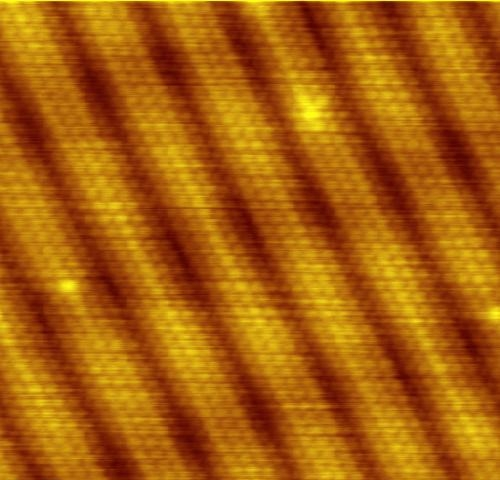
\includegraphics[width=0.6\linewidth]{Atomic_resolution_Au100.JPG}
	\caption{STM-bilde av 100-planet til gull som viser rekonstruksjon på overflaten. Atomene ordner seg i kolonner med tykkelse på noen få atomer, med gap mellom hver kolonne.}
	\label{fig:recAu}
\emd\end{figure}

I Figur \ref{fig:recAu} har man kuttet langs (100)-planet. Hvis man i stedet kutter langs (111)-planet, som har en heksagonal struktur, vil det i stedet dannes en fiskebein-struktur. Ved likevekt er det 23 overflateatomer på en avstand som tilsvarer 22 atomer i bulk, og dette kompenserer materialet for ved å lage ``folder'' slik at noen atomer er hevet med \SI{0.03}{\nano\meter} i forhold til noen andre atomer.

Både relaksasjon og rekonstruksjon fører at det oppstår mekanisk spenning, siden overflateatomene blir strukket eller sammentrukket i forhold til atomplanene under overflaten. Dette er analogt med overflatespenning for væsker. %

\paragraph{Vicinale overflater} Her er en fin måte å lage overflater med relativt lang periodisitet på: kutt en krystall langs et plan som er tettpakket, men bom med en vinkel $\theta$ mellom \SI{0}{\degree} og \SI{15}{\degree}. Siden det er vanskelig å kutte gjennom atomer, vil du få den beste mulige tilnærmingen: en atomær trapp der trinnene har høyde på ett atom og lengde på $L = \frac{d}{\tan\theta}$, som vist i Figur \ref{fig:vicinal}. 
\begin{figure}[H]
	\bmd\centering
	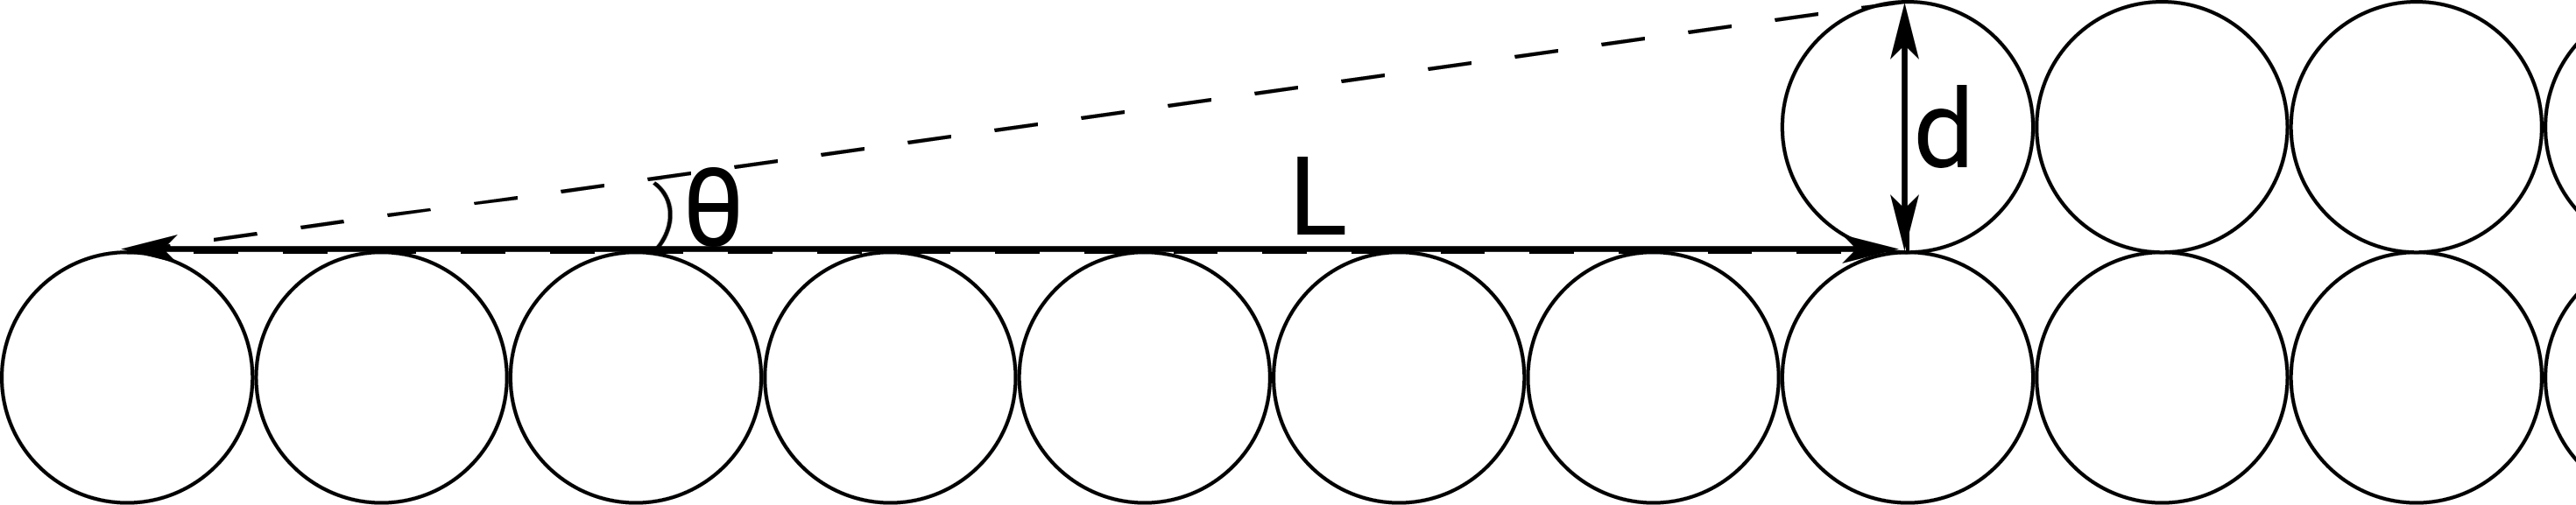
\includegraphics[width=\linewidth]{vicinal.png}
	\caption{Vicinal overflate}
	\label{fig:vicinal}
\emd\end{figure}
Gjennom en prosess som kalles fasettering vil overflaten så organisere seg på en måte som minimerer den frie energien i systemet.

Ved å stille inn $\theta$ slik du vil får du altså en periodisk struktur med rekker av atomer som er litt mer reaktive enn sine naboer (siden de er på en kant og ikke bare på en overflate), adskilt fra hverandre med et mellomrom på $L$.

% Det med oksygen og kobber
\paragraph{Kunstig mønstring} I tillegg til naturlige metoder for å lage mønstrede overflater kan vi også bruke litografi eller etsing til å lage mønstrede overflater.

\cstitletwo{Organisert vekst på et strukturert substrat}
Når man så lar materialet sitt adsorberes på substratet (ved en av metodene i neste delkapittel) kan vekst skje på tre måter, avhengig av balansen i fri energi mellom det adsorberte materialet (heretter adsorbatet), substratet og grenseflaten mellom de to. Dersom
\begin{equation}
	\gamma_{\text{substrat}} > \gamma_{\text{adsorbat}} + \gamma_{\text{grenseflate}}
\end{equation}
vil det første atomlaget av adsorbatet dekke hele substratet. La oss så kalle den nye frie energien for $\gamma_{\text{substrat}}'$, som nå tar hensyn til det nye laget av adsorbat og eventuelle stablefeil og dislokasjoner. Dersom vi nå har at 
\begin{equation}
	\gamma_{\text{substrat}}' > \gamma_{\text{adsorbat}} + \gamma_{\text{grenseflate}}
\end{equation}
vil påfølgende atomlag fortsette å dekke hele substratet, og adsorbatet dannes lag for lag. Denne typen vekst kalles FM-vekst (etter Frank-van der Merve), og er ikke så veldig interessant. 

Hvis $\gamma_{\text{substrat}}'$ derimot har blitt tilstrekkelig redusert, vil adsorbatet i stedet organisere seg i form av tredimensjonale klynger/øyer på toppen av det første laget. Denne typen vekst kalles \emph{Stranski-Krastanov}-vekst (SK-vekst på kort).

Dersom vi i utgangspunktet har 
\begin{equation}
	\gamma_{\text{substrat}} < \gamma_{\text{adsorbat}} + \gamma_{\text{grenseflate}}
\end{equation}
vil slike tredimensjonale klynger dannes direkte på substratet. Denne typen vekst kalles \emph{Volmer-Weber}-vekst (VW-vekst på kort). VW-vekst ser vi gjerne hvis et reaktivt materiale deponeres på et ikke-reaktivt substrat, for eksempel et overgangsmetall på et edelt metall.

I både SK- og VW-vekst dannes øyene gjennom nukleering og vekst. Atomene som når overflaten beveger seg rundt gjennom diffusjon, og det vil foregå nukleering der mange atomer møtes. Seinere i prosessen vil atomene begynne å sette seg på allerede eksisterende øyer i stedet for å begynne å lage nye øyer.

\cstitletwo{Vekst av indiumarsenid-kvanteprikker på galliumarsenid}

\paragraph{Balanse mellom overflateenergi/kurvatureffekter og elastisk energi} Det er en balanse mellom overflateenergi og elastisk energi som bestemmer hvordan øyene vokser. Man har et ledd i det kjemiske potensialet som avhenger av overflateenergi og forskyver likevekten mot vekst i konkave områder som groper og hull, men man har også et ledd assosiert med elastisk energi i bulk-atomene som forskyver likevekten mot vekst i konvekse områder som kanter og hjørner. % Skjønte ikke :(

Vi har eksempler på synteser der den ene eller den andre effekten dominerer. For eksempel: hvis vi vokser \ce{InAs} på \ce{GaAs} som man har laget sagtannform i ved å bruke interferometri og etse, vil vekst foregå på bunnen av de konkave områdene. Dette er fordi kurvatureffektene blir dominerende. Hvis vi derimot vokser \ce{InAs} på en flerlagsstruktur med \ce{In_{$x$}Ga_{$1-x$}As} mellom to lag av \ce{GaAs}, vil de elastiske effektene dominere slik at \ce{InAs} vokser på toppen av strukturen.

% MOAR!